\documentclass[../../master-handout.tex]{subfiles}

\begin{document}
\section{Lecture 19 (Wed, July 15)}
\sidenote{\textbf{Scribe:} Michael Zhou \\ \textbf{Date:} Wed, July 15, 2026}

\subsection{Unicycle Model and Lookahead Point}

Consider a unicycle at position $(p_x, p_y)$ with heading $\theta$, and a
\emph{lookahead point} (``end-effector'') placed a distance $\ell > 0$ ahead of
the vehicle along its heading. The goal position is $(p_{x,G},\, p_{y,G})$.

\begin{figure}[htbp]
    \centering
    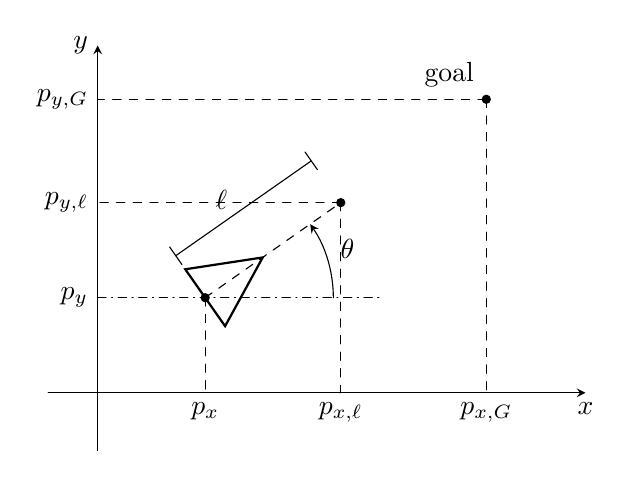
\begin{tikzpicture}[scale=1.05, >=stealth, line cap=round]
        % ---- axes ----
        \draw[->] (-0.6,0) -- (5.9,0) node[below] {$x$};
        \draw[->] (0,-0.7) -- (0,4.2) node[left] {$y$};

        % ---- projections onto the axes ----
        \draw[dashed] (1.30,1.15) -- (1.30,0);
        \draw[dashed] (2.94,2.30) -- (2.94,0);
        \draw[dashed] (4.70,3.55) -- (4.70,0);
        \draw[dashed] (2.94,2.30) -- (0,2.30);
        \draw[dashed] (4.70,3.55) -- (0,3.55);
        % horizontal reference through the robot
        \draw[dash dot] (0,1.15) -- (3.45,1.15);

        % ---- the unicycle, drawn as a wedge pointing along the heading ----
        \draw[thick] (1.059,1.494) -- (1.996,1.637) -- (1.541,0.806) -- cycle;
        % heading ray out to the lookahead point
        \draw[dashed] (1.30,1.15) -- (2.94,2.30);

        % ---- lookahead distance, as an offset dimension bar ----
        \draw (0.944,1.658) -- (2.583,2.805);
        \draw (1.019,1.551) -- (0.870,1.764);
        \draw (2.657,2.699) -- (2.508,2.912);
        \node at (1.495,2.336) {$\ell$};

        % ---- heading angle ----
        \draw[->] (2.85,1.15) arc (0:35:1.55);
        \node at (3.02,1.74) {$\theta$};

        % ---- markers ----
        \fill (1.30,1.15) circle (1.6pt);
        \fill (2.94,2.30) circle (1.6pt);
        \fill (4.70,3.55) circle (1.6pt) node[above left=1pt] {goal};

        % ---- axis labels ----
        \node[below] at (1.30,0) {$p_x$};
        \node[below] at (2.94,0) {$p_{x,\ell}$};
        \node[below] at (4.70,0) {$p_{x,G}$};
        \node[left] at (0,1.15) {$p_y$};
        \node[left] at (0,2.30) {$p_{y,\ell}$};
        \node[left] at (0,3.55) {$p_{y,G}$};
    \end{tikzpicture}
    \caption{The unicycle at $(p_x,p_y)$ with heading $\theta$, its lookahead
    point at distance $\ell$, and the goal $(p_{x,G}, p_{y,G})$.}
    \label{fig:unicycle-lookahead}
\end{figure}

The lookahead point is
\begin{equation}
    \begin{cases}
        p_{x,\ell} = p_x + \ell \cos\theta, \\
        p_{y,\ell} = p_y + \ell \sin\theta,
    \end{cases}
    \label{eq:lookahead}
\end{equation}
and the unicycle kinematics are
\begin{equation}
    \begin{cases}
        \dot{p}_x = v \cos\theta, \\
        \dot{p}_y = v \sin\theta, \\
        \dot{\theta} = \omega,
    \end{cases}
    \label{eq:unicycle}
\end{equation}
with inputs $v$ (forward speed) and $\omega$ (turning rate).

Differentiating \eqref{eq:lookahead} along \eqref{eq:unicycle}:
\begin{equation}
    \begin{cases}
        \dot{p}_{x,\ell} = \dot{p}_x - \ell \sin\theta \, \dot{\theta}
            = v\cos\theta - \ell \sin\theta \, \omega, \\
        \dot{p}_{y,\ell} = \dot{p}_y + \ell \cos\theta \, \dot{\theta}
            = v\sin\theta + \ell \cos\theta \, \omega.
    \end{cases}
\end{equation}

In matrix form,
\begin{fullwidth}
\begin{equation}
    \begin{bmatrix} \dot{p}_{x,\ell} \\ \dot{p}_{y,\ell} \end{bmatrix}
    =
    \begin{bmatrix}
        \cos\theta & -\ell\sin\theta \\
        \sin\theta & \ell\cos\theta
    \end{bmatrix}
    \begin{bmatrix} v \\ \omega \end{bmatrix}
    =
    \underbrace{
    \begin{bmatrix}
        \cos\theta & -\sin\theta \\
        \sin\theta & \cos\theta
    \end{bmatrix}}_{R(\theta)}
    \underbrace{
    \begin{bmatrix} 1 & 0 \\ 0 & \ell \end{bmatrix}}_{L}
    \begin{bmatrix} v \\ \omega \end{bmatrix}.
    \label{eq:RL}
\end{equation}
\end{fullwidth}

The matrix $R(\theta) L$ is invertible for every $\theta$ whenever
$\ell \neq 0$, so the lookahead point is \emph{fully actuated}: we can assign
any desired velocity to it.

\subsection{Control Law}

\textbf{Assign your favourite dynamics} to
$\begin{bmatrix} \dot{p}_{x,\ell} & \dot{p}_{y,\ell} \end{bmatrix}^\top$. The
simplest choice is a proportional law toward the goal, with gain $K > 0$:
\begin{equation}
    \begin{bmatrix}
        K \left(p_{x,G} - p_{x,\ell}\right) \\
        K \left(p_{y,G} - p_{y,\ell}\right)
    \end{bmatrix}
    =
    \begin{bmatrix} \dot{p}_{x,\ell} \\ \dot{p}_{y,\ell} \end{bmatrix}
    = R(\theta) \, L \begin{bmatrix} v \\ \omega \end{bmatrix}.
\end{equation}

Inverting \eqref{eq:RL} (using $R^{-1} = R^\top$) gives the unicycle inputs:
\begin{fullwidth}
\begin{equation}
    \begin{bmatrix} v \\ \omega \end{bmatrix}
    = L^{-1} R(\theta)^{-1}
    \begin{bmatrix}
        K \left(p_{x,G} - p_{x,\ell}\right) \\
        K \left(p_{y,G} - p_{y,\ell}\right)
    \end{bmatrix}
    =
    \begin{bmatrix} 1 & 0 \\ 0 & \frac{1}{\ell} \end{bmatrix}
    R(\theta)^\top
    \begin{bmatrix}
        K \left(p_{x,G} - p_{x,\ell}\right) \\
        K \left(p_{y,G} - p_{y,\ell}\right)
    \end{bmatrix}.
    \label{eq:control}
\end{equation}
\end{fullwidth}

Under this control, the lookahead point converges exponentially to the goal.

\subsection{From $(v, \omega)$ to Differential-Drive Wheel Speeds}

A differential-drive robot with wheel separation $d$ and wheel radius $r$ is
kinematically equivalent to the unicycle. Its left/right wheel ground speeds
are $v_L = \omega_L \cdot r$ and $v_R = \omega_R \cdot r$, where
$\omega_L, \omega_R$ are the wheel angular rates.

\begin{figure}[htbp]
    \centering
    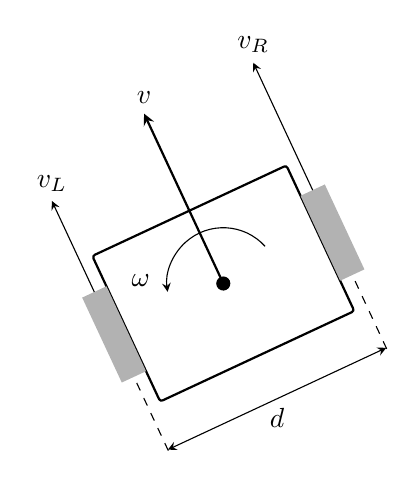
\begin{tikzpicture}[scale=1.7, >=stealth, rotate=25]
        \draw[thick, rounded corners=1pt] (-0.8,-0.6) rectangle (0.8,0.6);
        \fill[gray!60] (-1.0,-0.35) rectangle (-0.8,0.35);
        \fill[gray!60] (0.8,-0.35) rectangle (1.0,0.35);
        \fill (0,0) circle (1.5pt);
        \draw[->, thick] (0,0) -- (0,1.4) node[above] {$v$};
        \draw[->] (0.4,0.12) arc (17:163:0.42);
        \node at (-0.55,0.28) {$\omega$};
        \draw[->] (-0.9,0.35) -- ++(0,0.75) node[above] {$v_L$};
        \draw[->] (0.9,0.35) -- ++(0,1.05) node[above] {$v_R$};
        \draw[dashed] (-0.9,-0.4) -- (-0.9,-1.0);
        \draw[dashed] (0.9,-0.4) -- (0.9,-1.0);
        \draw[<->] (-0.9,-0.95) -- (0.9,-0.95) node[midway, below] {$d$};
    \end{tikzpicture}
    \caption{Differential-drive robot with wheel separation $d$, forward speed
    $v$, turning rate $\omega$, and wheel speeds $v_L$ and $v_R$.}
    \label{fig:diff-drive}
\end{figure}

The wheel speeds relate to the unicycle inputs by
\begin{equation}
    \begin{cases}
        v_L = v - \dfrac{d}{2}\,\omega, \\[1.2ex]
        v_R = v + \dfrac{d}{2}\,\omega,
    \end{cases}
    \qquad \Longleftrightarrow \qquad
    \begin{bmatrix} v_L \\ v_R \end{bmatrix}
    =
    \underbrace{
    \begin{bmatrix}
        1 & -\frac{d}{2} \\
        1 & \frac{d}{2}
    \end{bmatrix}}_{D}
    \begin{bmatrix} v \\ \omega \end{bmatrix}.
\end{equation}

Composing with the controller of the previous section, the wheel-speed commands
are
\begin{fullwidth}
\begin{equation}
    \boxed{\;
    \begin{bmatrix} v_L \\ v_R \end{bmatrix}
    = D \, L^{-1} R(\theta)^\top
    \begin{bmatrix}
        K \left(p_{x,G} - p_{x,\ell}\right) \\
        K \left(p_{y,G} - p_{y,\ell}\right)
    \end{bmatrix}. \;}
\end{equation}
\end{fullwidth}

\subsection{Near-Identity Diffeomorphism}

The lookahead construction is an instance of a general idea.

\paragraph{Definition.}
Let
\begin{equation}
    \Psi : \R^n \times \R^p \longrightarrow \R^n \quad \text{smooth}, \qquad
    p = \Psi(x, \ell),
\end{equation}
be a \emph{global diffeomorphism in $x$} for every $\ell \in \R^p$. Then $\Psi$
is a \textbf{near-identity diffeomorphism} if
\begin{equation}
    \forall\, x \in \R^n: \qquad \Psi(x, \ell) = x \iff \ell = 0,
\end{equation}
i.e.\ $\ell = 0 \iff \Psi(x, 0) = x$ (the map reduces to the identity, $p = x$).

\paragraph{Example.}
The lookahead map used above,
\begin{equation}
    p = x + \ell \begin{bmatrix} \cos\theta \\ \sin\theta \end{bmatrix},
    \qquad
    p = \begin{bmatrix} p_{x,\ell} \\ p_{y,\ell} \end{bmatrix},
    \qquad
    x = \begin{bmatrix} p_x \\ p_y \end{bmatrix},
\end{equation}
is a near-identity diffeomorphism: for $\ell = 0$ it reduces to
$\Psi(x, 0) = x$, and for $\ell \neq 0$ it shifts the state by a fixed offset
along the heading, which is invertible in $x$.

Went to watch world cup!

\end{document}
